\documentclass[11pt]{article}
\usepackage[top=1.00in, bottom=1.0in, left=1in, right=1in]{geometry}
\renewcommand{\baselinestretch}{1.1}
\usepackage{graphicx}
\usepackage{natbib}
\usepackage{amsmath}
\usepackage{parskip}

\def\labelitemi{--}
\parindent=0pt

\begin{document}
\bibliographystyle{/Users/Lizzie/Documents/EndnoteRelated/Bibtex/styles/besjournals}
\renewcommand{\refname}{\CHead{}}

% \setlength{\parindent}{0cm}
% \setlength{\parskip}{5pt}

\section*{Overview}

We propose follow simple example of Wade 2000 (with citation to it) with a climate change twise... 
\begin{itemize}
\item Back story for our example ... 
\begin{itemize}
\item Imagine you have sampled 10 populations of a species across its latitudinal range
\item Populations are increasing at the leading edge, but declining fast at the trailing edge.
\item However, there's different sample sizes (years of data) at each site and there happens to be much less at the most trailing edge population
\end{itemize}
\item What we'll do. ... 
\begin{itemize}
\item We'll simulate from a basic logistic growth model and add equal noise across all populations, then reduce the sample size ($n$ of years) variably but the most for the most trailing and make sure one a little up of that has LOTS of data
\item We'll show trends lines with error and asterisks for the NHT look and each one will be paired with a posterior with 0 highlighted by a dashed line ({\bf we could also show the true slope?} Though I am not sure how to calculate that ... given the underlying model is non-linear, but we could estimate on the data without the noise added). We will make sure the $x$ axis is the same across all the posteriors so the decline is apparent. 
\end{itemize}
\item What this will show ... 
\begin{itemize}
\item The most declining population will not have a significant slope so will not be flagged for concern under NHT and p-values but will look concerning with the posterior.
\item Instead the NHT will make the well sampled but barely declining population look most concerning. 
\end{itemize}
\end{itemize}

\newpage
\section*{Text for box}

In some cases, Bayesian approaches can lead to importantly different conclusions than common Fisherian approaches, such as null hypothesis testing (Wade 2000). Consider, for example, sampling five populations of a species across its range---from north to south---to monitor for changes in the population size with climate change. After collecting data for ten years, a traditional null hypothesis testing approach to analyzing the data, using the common Type I error value ($\alpha$) of 0.05 would find changes in only two of the populations---the furthest north population, which appears to be increasing, and the second furthest north population, also increasing. The three other populations are not significantly changing under this approach (Fig. \refl{fig:nht} left). In contrast, a Bayesian approach (using weakly informative priors centered at zero, all code provided in supplement) would likely focus on the posteriors, where small differences in the variance do not appear so different  (Fig. \refl{fig:nht} right). Here, a a clear trend emerges where trends in population correlate with position in range---with the most northern population increasing the most and the most southern population decreasing the most. This pattern across the range is the type predicted by climate change and may be missed with a classic Fisherian approach (combining null hypothesis testing with threshold values for `significance'), leading to potential very difference conservation and management decisions. % EMW says: We could also add (1) more details on the simulations (the variance in the underlying model increases going from north to south, which is expected for smaller population sizes), (2) point out 10 years is often more years than we have; though I think there is enough text already. 

\begin{figure}
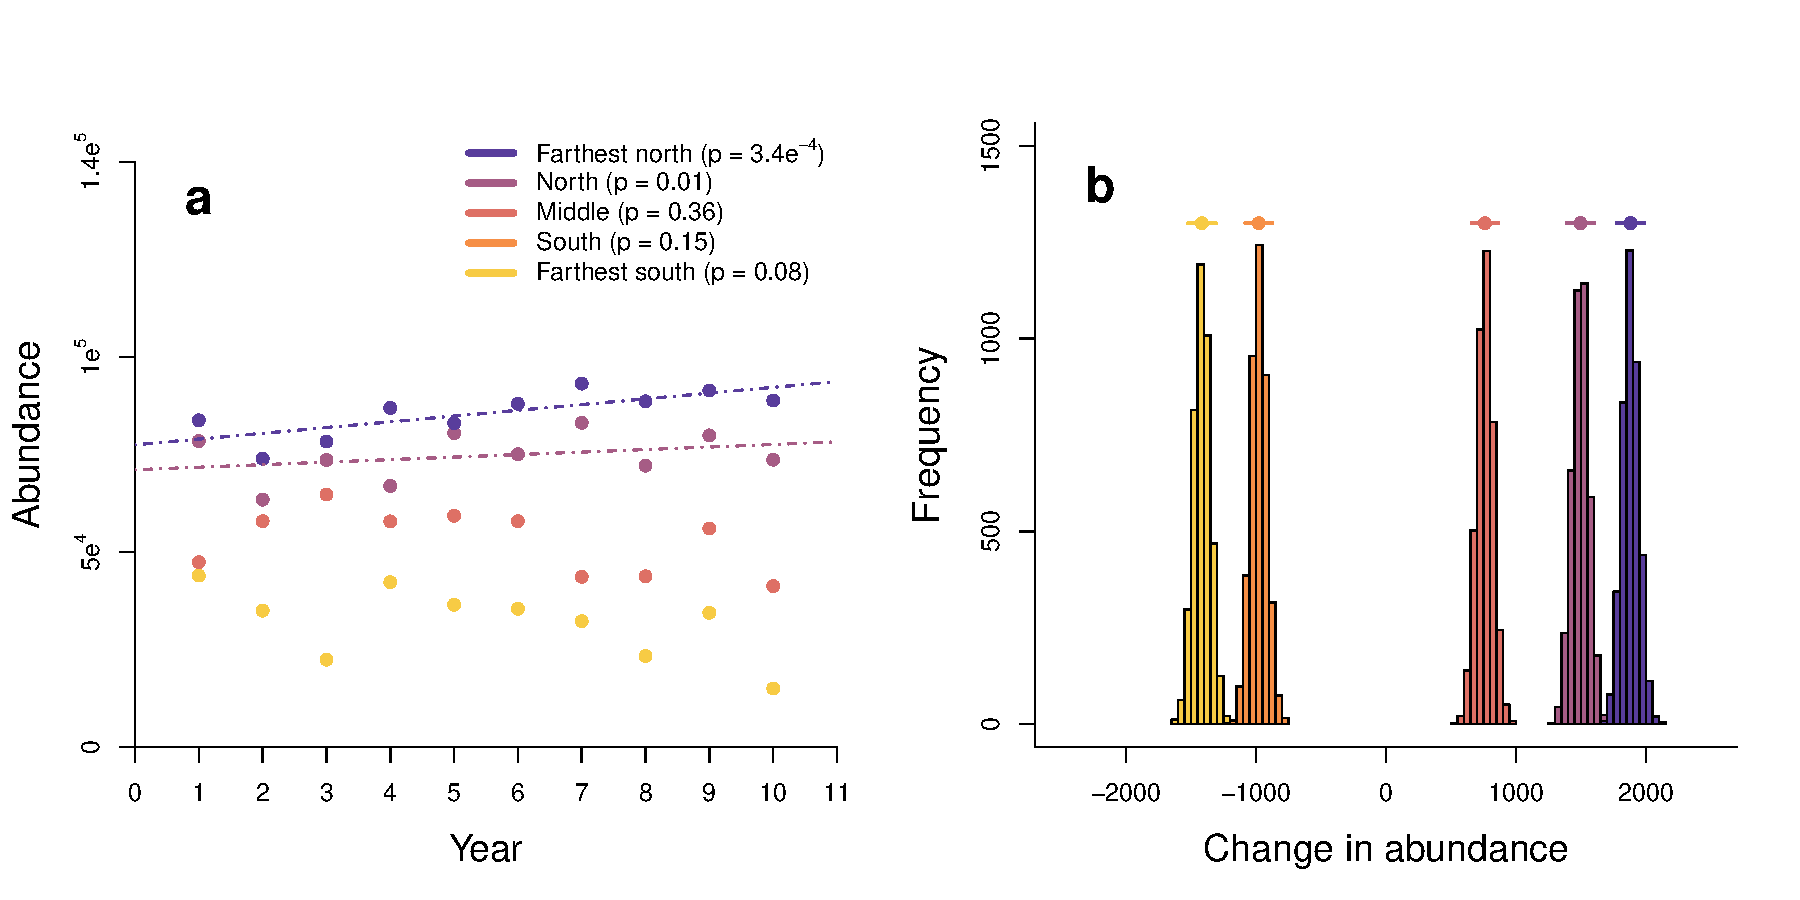
\includegraphics[width=1\textwidth]{figures/nhtBoxLayeredMeans.pdf}
\caption{Trends in population size over time (left) analyzed with a traditional Fisherian approach using null hypothesis testing (using an $\alpha$ of 0.05 to reject the null hypothesis of a slope of zero) versus a Bayesian approach, which focuses on the posterior distribution (right).}
\label{fig:nht}
\end{figure}

\end{document}

